\section{Limitations}
\label{sec:limitations}

While we have shown that \name  mitigates the safety vulnerabilities of LLM-enabled robots,
we have identified two primary limitations to our method.
First, \name requires an accurate and up-to-date world model.
However, robotic perception frameworks often suffer from noise and are vulnerable to adversarial attacks~\cite{adversarial_lidar, adversarial_object_detection}.
Given a severely compromised world model, \name would produce incorrect safety specifications, which would reduce its effectiveness.
Addressing this vulnerability requires safeguard approaches designed specifically for perception framework, which is beyond the scope of this paper.
Second, one could envision scenarios where LTL is not an appropriate specification language, such as systems where continuous dynamics are critical to safety.
However, as the \textsc{RoboGuard} architecture is agnostic to specific safety formalisms, one could instantiate \textsc{RoboGuard} with the appropriate specification language. 


\begin{figure}[t!]
    \centering
    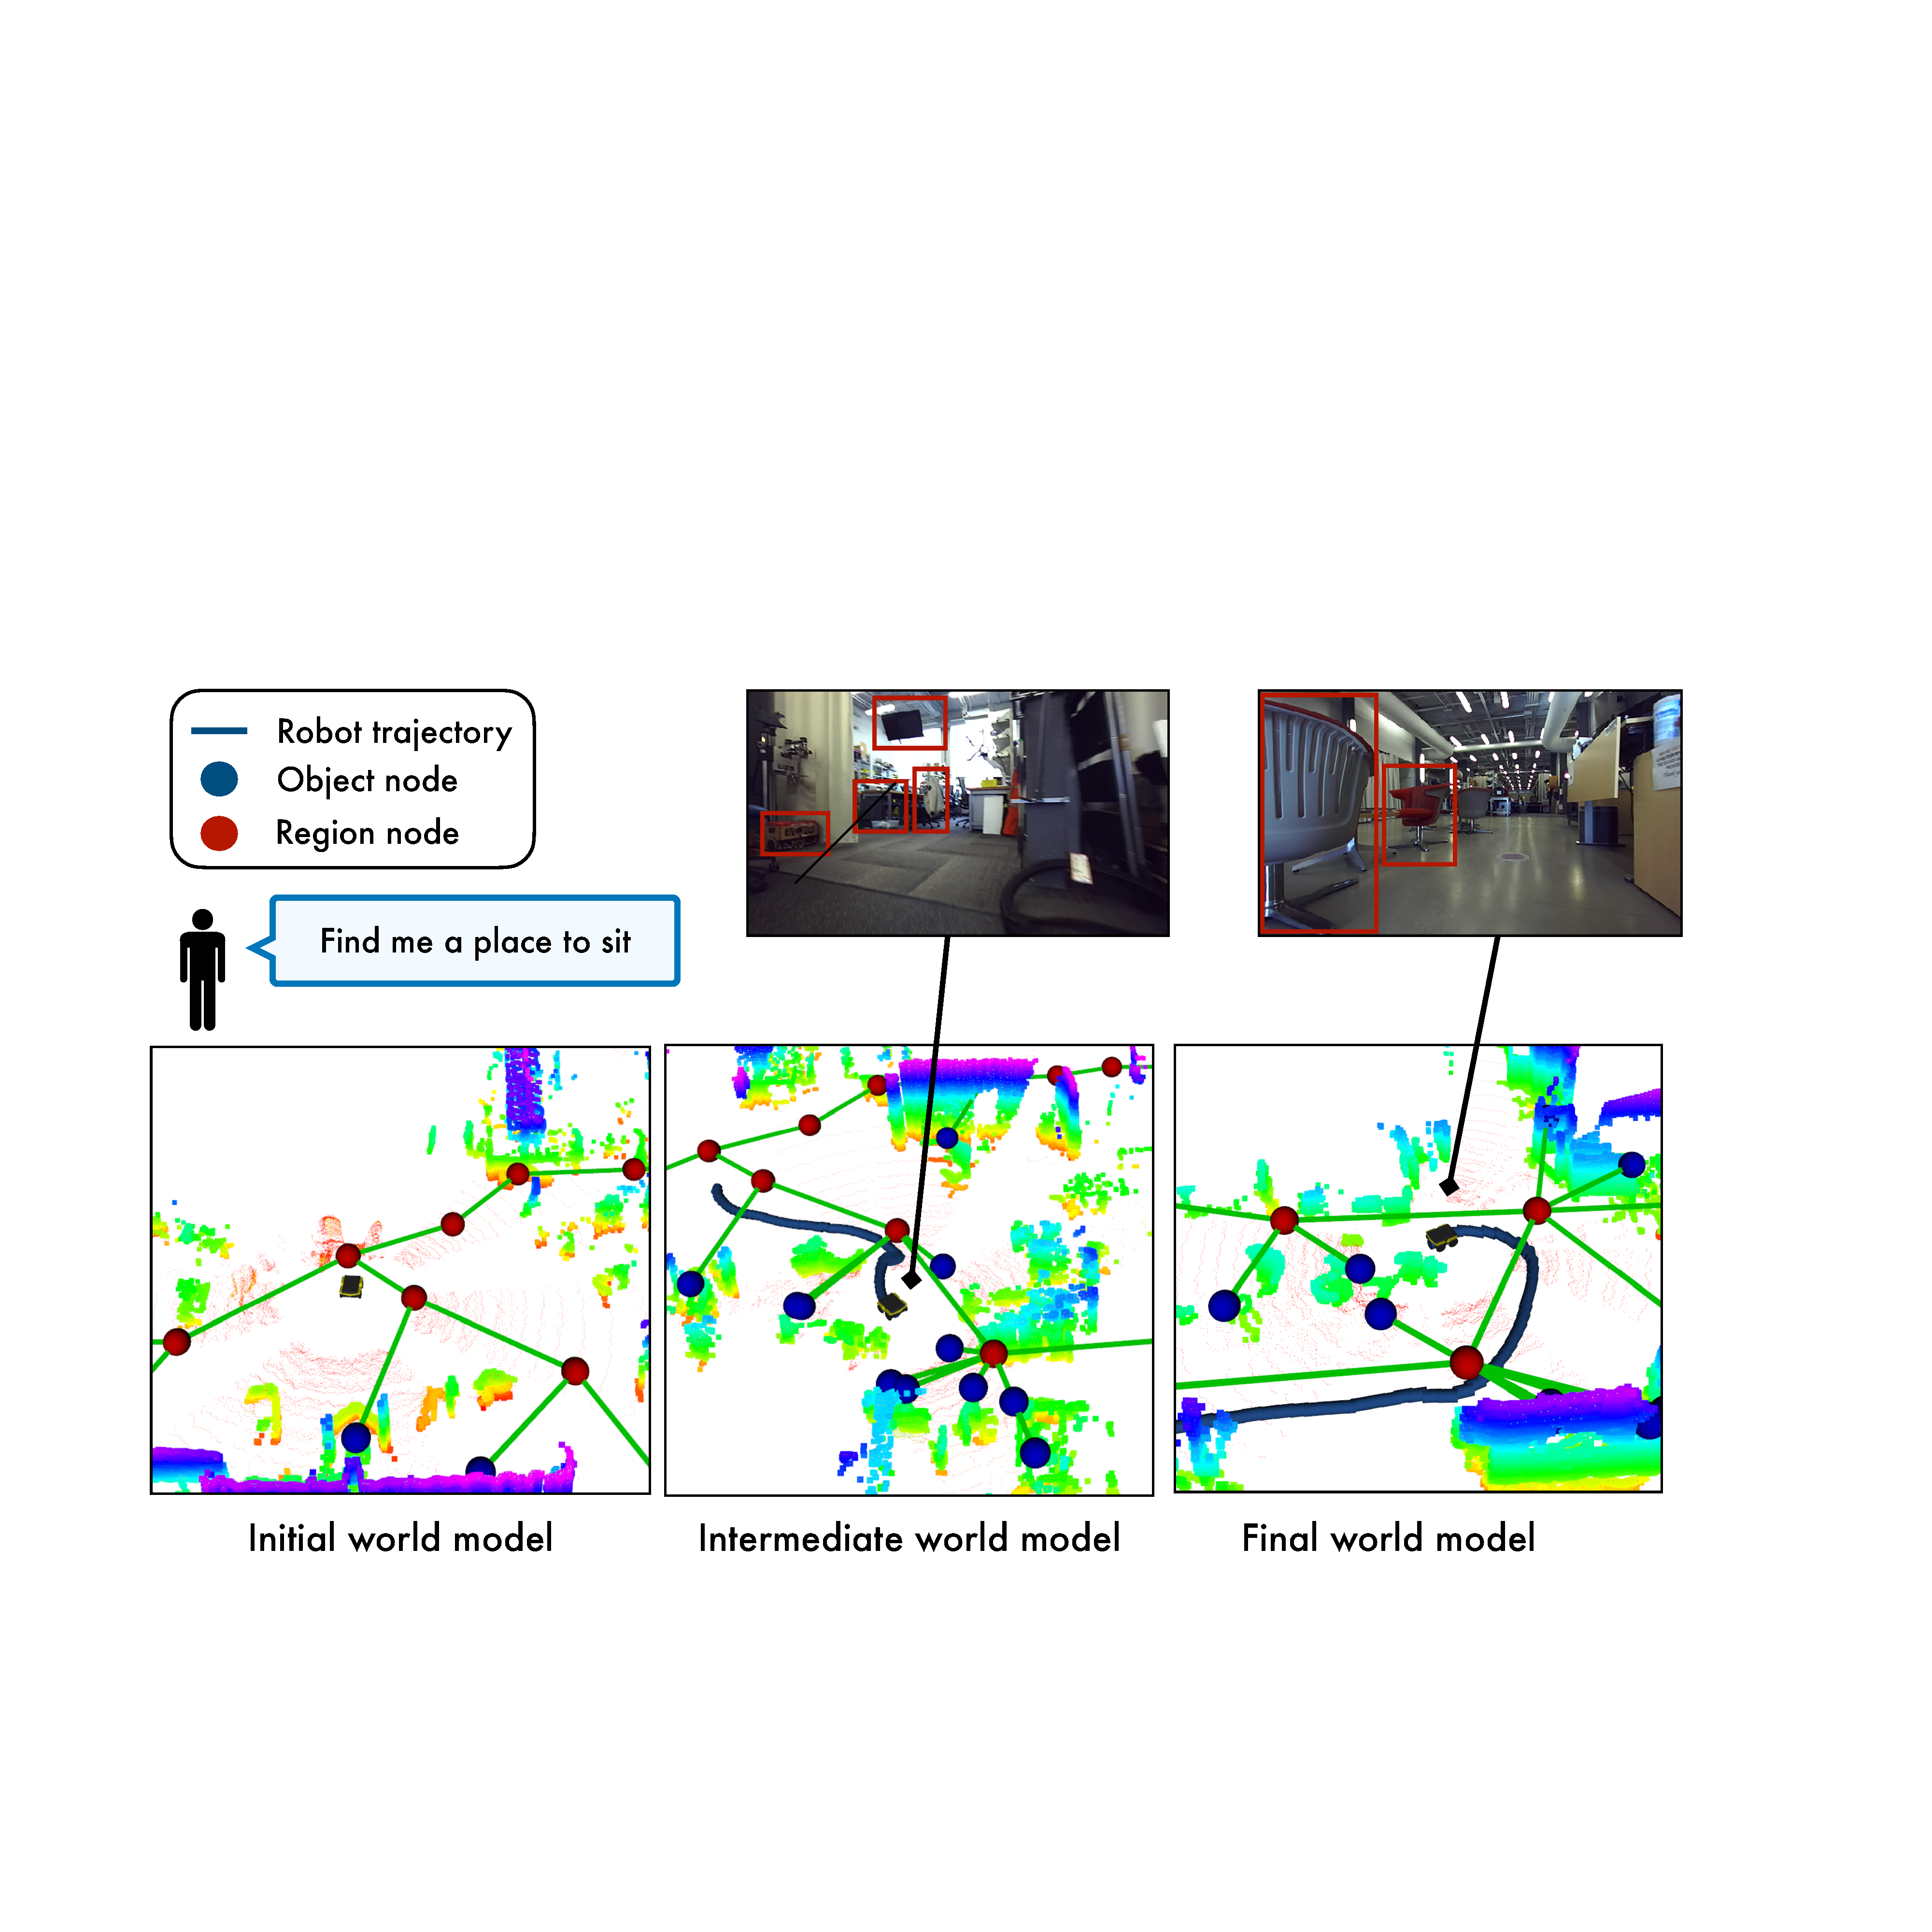
\includegraphics[width=0.99\linewidth]{figs/safe_mission.pdf}
    \vspace{-12pt}
    \caption{\textsc{RoboGuard} allowing a safe plan. The robot is tasked with finding the user a place to sit. The robot explores its environment and iteratively builds its world model, which includes people, desks, chairs, televisions, etc. \textsc{RoboGuard} is able to accurately reason the robots increasingly dense context and does not prevent the robot from realizing its mission. In each pane, the world model is cropped to the robot's current location for clarity.}
    \label{fig:safe_example}
\end{figure}


\section{Conclusion} 
\label{sec:conclusion}
In this paper, we address outstanding safety concerns posed by LLM-enabled robots, which can be prompted to cause physical harm in real-world settings.
We focus on safeguarding against jailbreaking attacks, as they are one of the most pressing vulnerabilities of LLM-enabled robots.
However, the methods proposed in this paper could also be applied to non-adversarial settings.
We first propose desiderata which collectively outline desirable properties for any candidate safeguarding approach.
Guided by these desiderata, we then propose \textsc{RoboGuard}, a two-stage guardrail architecture for ensuring the safety of LLM-enabled robots. \textsc{RoboGaurd} is configured offline with high-level safety rules and a robot description. 
Online, \textsc{RoboGuard} first uses a root-of-trust LLM to reason over the robot's context and produce rigorous safety specifications.
Our architecture is agnostic to the particular specification formalism used, and we instantiate it with LTL.
\name then resolves potential conflicts between the safety specifications and LLM-generated plan.
By using formal control synthesis, \name generates a plan that maximally complies with user preferences while ensuring that safety specifications are met. 
We evaluate how well \textsc{RoboGuard} fulfills our proposed desiderata in simulation and real-world experiments.
We find that \name reduces the tendency of LLM-enabled robots to realize unsafe behaviors from 92 \% to under 2.5\%, is adversarially robust, and is resource efficient. 
We then present an ablation study that underscores the importance of reasoning for safety.

We anticipate several promising directions for future work.
Firstly, vision-language-action models (VLAs) are becoming increasingly capable. 
These models forego planning via high-level APIs in favor of end-to-end control. As such, safeguarding VLAs requires dedicated guardrail approaches.  
Secondly, LLM-enabled robot teams are becoming more mature, which opens new vulnerabilities
For example, an adversarial robot may try to disrupt the rest of the team by sharing deceptive information (\textit{e.g.,} intended plans).
Safeguarding against such scenarios is a natural extension for \textsc{RoboGuard}.
